% generated by gen_arch_v2.py -- do not edit by hand
\documentclass[10pt]{standalone}
\usepackage{mathptmx}
\usepackage{tikz}
\usetikzlibrary{arrows.meta}
\definecolor{cctl}{HTML}{FFF2CC}
\definecolor{ciss}{HTML}{DDEBF7}
\definecolor{cexe}{HTML}{E4DFEC}
\definecolor{csto}{HTML}{E2EFDA}
\definecolor{cmem}{HTML}{FBE5D6}
\definecolor{chl}{HTML}{F8CBAD}
\definecolor{chlb}{HTML}{C55A11}
\definecolor{cps}{HTML}{EDEDED}
\newcommand{\fsz}{\fontsize{6.5}{7.5}\selectfont}
\begin{document}
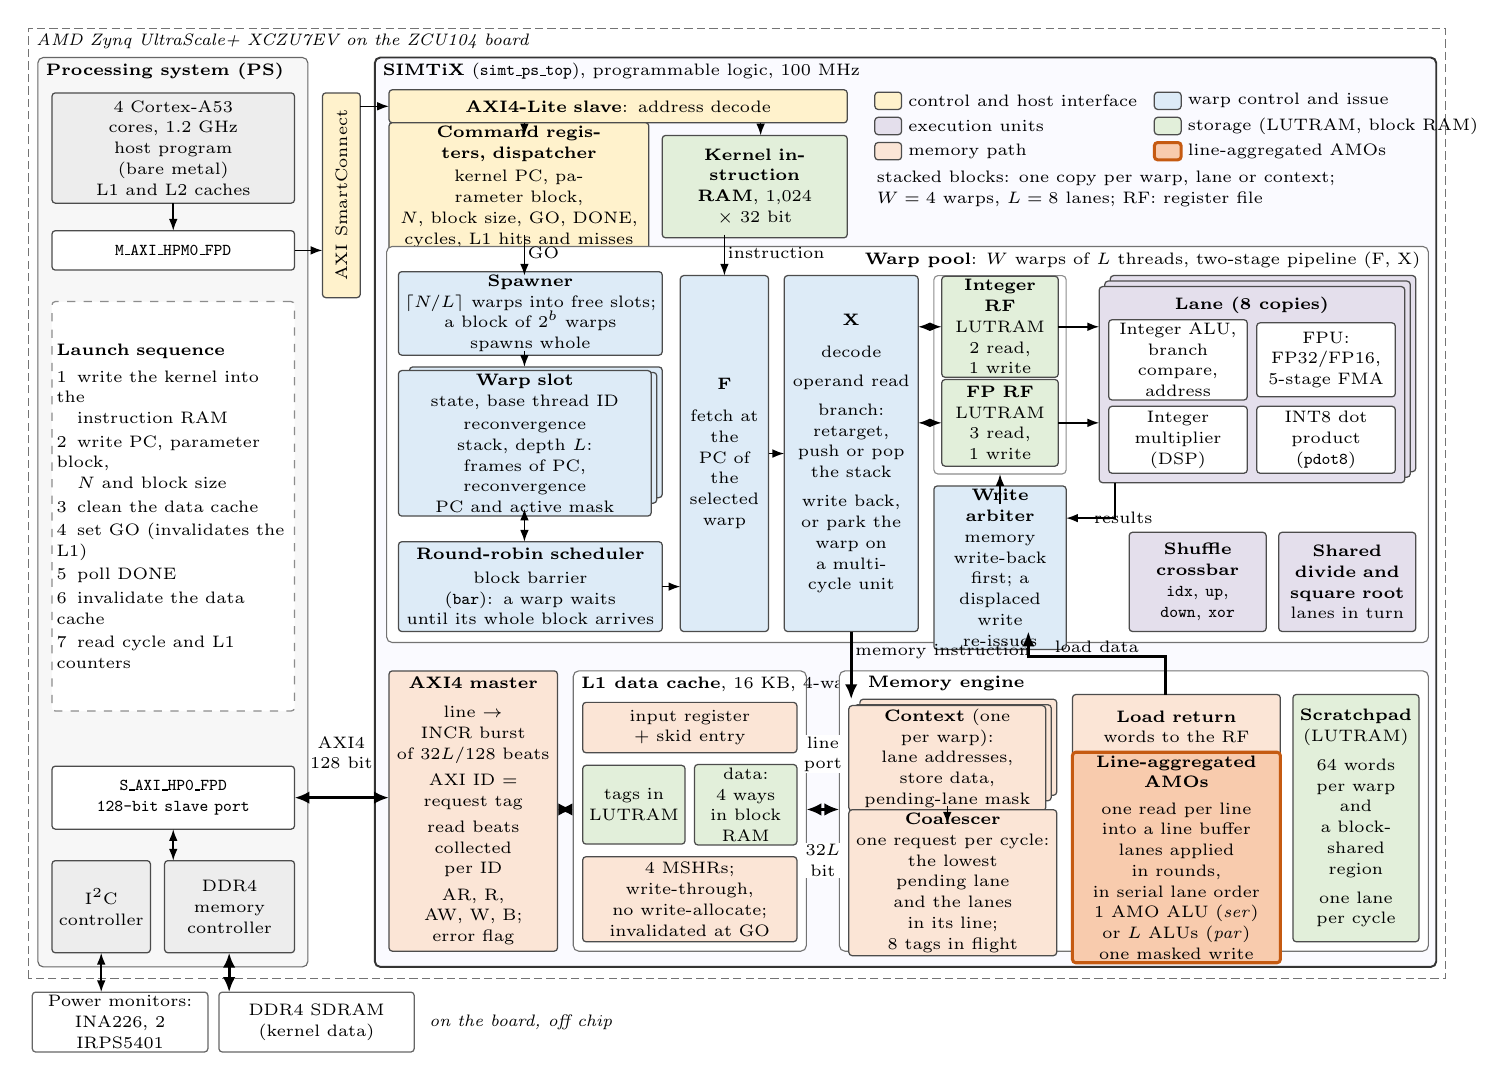
\begin{tikzpicture}[x=1cm, y=1cm,
  base/.style={draw=black!70, rounded corners=1.2pt, align=center, font=\fsz,
               inner sep=1.2pt, line width=0.45pt},
  ctl/.style={base, fill=cctl},   ctlbox/.style={base, fill=cctl},
  iss/.style={base, fill=ciss},   issbox/.style={base, fill=ciss},
  exe/.style={base, fill=cexe},   exebox/.style={base, fill=cexe},
  exein/.style={base, fill=white},
  sto/.style={base, fill=csto},   stobox/.style={base, fill=csto},
  mem/.style={base, fill=cmem},   membox/.style={base, fill=cmem},
  hl/.style={base, fill=chl, draw=chlb, line width=1.1pt},
  hlbox/.style={base, fill=chl, draw=chlb, line width=1.1pt},
  ps/.style={base, fill=cps},
  port/.style={base, fill=white, font=\fsz\ttfamily},
  note/.style={base, fill=white, draw=black!45, dashed, align=left},
  off/.style={base, fill=white, draw=black!60},
  devframe/.style={draw=black!55, line width=0.5pt, dash pattern=on 3pt off 1.5pt},
  psframe/.style={draw=black!60, fill=black!3, rounded corners=2pt},
  accframe/.style={draw=black!80, fill=blue!2, rounded corners=2pt, line width=0.7pt},
  wpframe/.style={draw=black!55, fill=white, rounded corners=2pt},
  memframe/.style={draw=black!55, fill=white, rounded corners=2pt},
  rfframe/.style={draw=black!45, fill=white, rounded corners=1.5pt},
  flabel/.style={font=\fsz, inner sep=1pt},
  dlabel/.style={font=\fsz\itshape, inner sep=1pt},
  olabel/.style={font=\fsz\itshape, inner sep=1pt},
  lgtext/.style={font=\fsz, inner sep=0.5pt},
  elabel/.style={font=\fsz, inner sep=1pt},
  arr/.style={-{Latex[length=1.5mm, width=1.1mm]}, line width=0.55pt},
  darr/.style={{Latex[length=1.5mm, width=1.1mm]}-{Latex[length=1.5mm, width=1.1mm]},
               line width=0.55pt},
  bus/.style={-{Latex[length=1.9mm, width=1.6mm]}, line width=1.1pt},
  bdarr/.style={{Latex[length=1.9mm, width=1.6mm]}-{Latex[length=1.9mm, width=1.6mm]},
                line width=1.1pt}]
\draw[devframe] (0.000,0.950) rectangle (18.000,13.020);
\node[dlabel, anchor=north west] at (0.060,12.990) {AMD Zynq UltraScale+ XCZU7EV on the ZCU104 board};
\draw[psframe] (0.120,1.100) rectangle (3.550,12.650);
\node[flabel, anchor=north west] at (0.180,12.620) {\textbf{Processing system (PS)}};
\draw[accframe] (4.400,1.100) rectangle (17.880,12.650);
\node[flabel, anchor=north west] at (4.460,12.620) {\textbf{SIMTiX} (\texttt{simt\_ps\_top}), programmable logic, 100~MHz};
\node[ps, minimum width=3.080cm, minimum height=1.400cm, text width=2.960cm] (a53) at (1.840,11.500) {4 Cortex-A53 cores, 1.2~GHz\\host program (bare metal)\\L1 and L2 caches};
\node[port, minimum width=3.080cm, minimum height=0.500cm, text width=2.960cm] (hpm) at (1.840,10.200) {M\_AXI\_HPM0\_FPD};
\node[note, minimum width=3.080cm, minimum height=5.200cm, text width=2.960cm] (seq) at (1.840,6.950) {\textbf{Launch sequence}\\[2pt]1\enspace write the kernel into the\\\phantom{1}\enspace instruction RAM\\[1pt]2\enspace write PC, parameter block,\\\phantom{1}\enspace $N$ and block size\\[1pt]3\enspace clean the data cache\\[1pt]4\enspace set GO (invalidates the L1)\\[1pt]5\enspace poll DONE\\[1pt]6\enspace invalidate the data cache\\[1pt]7\enspace read cycle and L1 counters};
\node[port, minimum width=3.080cm, minimum height=0.800cm, text width=2.960cm] (hp0) at (1.840,3.250) {S\_AXI\_HP0\_FPD\\128-bit slave port};
\node[ps, minimum width=1.250cm, minimum height=1.170cm, text width=1.130cm] (i2c) at (0.925,1.865) {I$^2$C\\controller};
\node[ps, minimum width=1.650cm, minimum height=1.170cm, text width=1.530cm] (ddrc) at (2.555,1.865) {DDR4 memory\\controller};
\node[off, minimum width=2.230cm, minimum height=0.760cm, text width=2.110cm] (mon) at (1.165,0.400) {Power monitors:\\INA226, 2 IRPS5401};
\node[off, minimum width=2.480cm, minimum height=0.760cm, text width=2.360cm] (ddr) at (3.660,0.400) {DDR4 SDRAM (kernel data)};
\node[olabel, anchor=west] at (5.05,0.40) {on the board, off chip};
\node[ctl, minimum width=2.60cm, minimum height=0.48cm, rotate=90] (sc) at (3.975,10.90) {AXI SmartConnect};
\node[ctl, minimum width=5.820cm, minimum height=0.420cm, text width=5.700cm] (axil) at (7.490,12.030) {\textbf{AXI4-Lite slave}: address decode};
\node[ctl, minimum width=3.300cm, minimum height=1.300cm, text width=3.180cm] (regs) at (6.230,11.010) {\textbf{Command registers, dispatcher}\\[1pt]kernel PC, parameter block,\\$N$, block size, GO, DONE,\\cycles, L1 hits and misses};
\node[sto, minimum width=2.350cm, minimum height=1.300cm, text width=2.230cm] (iram) at (9.225,11.010) {\textbf{Kernel instruction}\\\textbf{RAM}, 1,024 $\times$ 32 bit};
\draw[ctlbox] (10.750,11.990) rectangle (11.090,12.210);
\node[lgtext, anchor=west] at (11.150,12.100) {control and host interface};
\draw[issbox] (14.300,11.990) rectangle (14.640,12.210);
\node[lgtext, anchor=west] at (14.700,12.100) {warp control and issue};
\draw[exebox] (10.750,11.670) rectangle (11.090,11.890);
\node[lgtext, anchor=west] at (11.150,11.780) {execution units};
\draw[stobox] (14.300,11.670) rectangle (14.640,11.890);
\node[lgtext, anchor=west] at (14.700,11.780) {storage (LUTRAM, block RAM)};
\draw[membox] (10.750,11.350) rectangle (11.090,11.570);
\node[lgtext, anchor=west] at (11.150,11.460) {memory path};
\draw[hlbox] (14.300,11.350) rectangle (14.640,11.570);
\node[lgtext, anchor=west] at (14.700,11.460) {line-aggregated AMOs};
\node[lgtext, anchor=west, align=left] at (10.75,10.98) {stacked blocks: one copy per warp, lane or context;\\$W=4$ warps, $L=8$ lanes; RF: register file};
\draw[wpframe] (4.550,5.220) rectangle (17.780,10.250);
\node[flabel, anchor=north east] at (17.72,10.22) {\textbf{Warp pool}: $W$ warps of $L$ threads, two-stage pipeline (F, X)};
\node[iss, minimum width=3.350cm, minimum height=0.960cm, text width=3.230cm] (spawn) at (6.375,9.400) {\textbf{Spawner}\\$\lceil N/L\rceil$ warps into free slots;\\a block of $2^b$ warps spawns whole};
\draw[issbox] (4.840,7.060) rectangle (8.050,8.720);
\draw[issbox] (4.770,6.990) rectangle (7.980,8.650);
\node[iss, minimum width=3.210cm, minimum height=1.660cm, text width=3.090cm] (slots) at (6.305,7.750) {\textbf{Warp slot}\\state, base thread ID\\[1pt]reconvergence stack, depth $L$:\\frames of PC, reconvergence\\PC and active mask};
\node[iss, minimum width=3.350cm, minimum height=1.140cm, text width=3.230cm] (sched) at (6.375,5.930) {\textbf{Round-robin scheduler}\\[1pt]block barrier (\texttt{bar}): a warp waits\\until its whole block arrives};
\node[iss, minimum width=1.120cm, minimum height=4.520cm, text width=1.000cm] (F) at (8.840,7.620) {\textbf{F}\\[4pt]fetch at\\the PC of\\the selected\\warp};
\node[iss, minimum width=1.700cm, minimum height=4.520cm, text width=1.580cm] (X) at (10.450,7.620) {\textbf{X}\\[4pt]decode\\[3pt]operand read\\[3pt]branch: retarget, push or pop the stack\\[3pt]write back, or park the warp on a multi-cycle unit};
\draw[rfframe] (11.500,7.360) rectangle (13.180,9.880);
\node[sto, minimum width=1.480cm, minimum height=1.100cm, text width=1.360cm] (irf) at (12.340,9.230) {\textbf{Integer RF}\\LUTRAM\\2 read, 1 write};
\node[sto, minimum width=1.480cm, minimum height=1.100cm, text width=1.360cm] (frf) at (12.340,8.010) {\textbf{FP RF}\\LUTRAM\\3 read, 1 write};
\node[iss, minimum width=1.680cm, minimum height=1.620cm, text width=1.560cm] (arb) at (12.340,6.170) {\textbf{Write arbiter}\\memory write-back first; a displaced write re-issues};
\draw[exebox] (13.740,7.390) rectangle (17.620,9.880);
\draw[exebox] (13.670,7.320) rectangle (17.550,9.810);
\node[exe, minimum width=3.880cm, minimum height=2.490cm, text width=3.760cm] (lane) at (15.540,8.495) {};
\node[font=\fsz\bfseries] at (15.54,9.50) {Lane (8 copies)};
\node[exein, minimum width=1.760cm, minimum height=0.940cm, text width=1.640cm] (alu) at (14.600,8.810) {Integer ALU,\\branch compare,\\address};
\node[exein, minimum width=1.760cm, minimum height=0.940cm, text width=1.640cm] (fpu) at (16.480,8.810) {FPU: FP32/FP16,\\5-stage FMA};
\node[exein, minimum width=1.760cm, minimum height=0.850cm, text width=1.640cm] (mul) at (14.600,7.795) {Integer\\multiplier (DSP)};
\node[exein, minimum width=1.760cm, minimum height=0.850cm, text width=1.640cm] (dot) at (16.480,7.795) {INT8 dot product\\(\texttt{pdot8})};
\node[exe, minimum width=1.740cm, minimum height=1.260cm, text width=1.620cm] (shfl) at (14.850,5.990) {\textbf{Shuffle crossbar}\\\texttt{idx}, \texttt{up},\\\texttt{down}, \texttt{xor}};
\node[exe, minimum width=1.740cm, minimum height=1.260cm, text width=1.620cm] (sfu) at (16.750,5.990) {\textbf{Shared divide and square root}\\lanes in turn};
\node[mem, minimum width=2.140cm, minimum height=3.560cm, text width=2.020cm] (axi) at (5.650,3.080) {\textbf{AXI4 master}\\[3pt]line $\to$ INCR burst\\of $32L/128$ beats\\[2pt]AXI ID = request tag\\[2pt]read beats collected\\per ID\\[2pt]AR, R, AW, W, B;\\error flag};
\draw[memframe] (6.920,1.300) rectangle (9.880,4.860);
\node[flabel, anchor=north west] at (6.980,4.830) {\textbf{L1 data cache}, 16~KB, 4-way};
\node[mem, minimum width=2.720cm, minimum height=0.640cm, text width=2.600cm] (inreg) at (8.400,4.140) {input register + skid entry};
\node[sto, minimum width=1.300cm, minimum height=1.000cm, text width=1.180cm] (tags) at (7.690,3.160) {tags in\\LUTRAM};
\node[sto, minimum width=1.300cm, minimum height=1.000cm, text width=1.180cm] (data) at (9.110,3.160) {data: 4 ways\\in block RAM};
\node[mem, minimum width=2.720cm, minimum height=1.080cm, text width=2.600cm] (mshr) at (8.400,1.960) {4 MSHRs; write-through,\\no write-allocate;\\invalidated at GO};
\draw[memframe] (10.300,1.300) rectangle (17.780,4.860);
\node[flabel, anchor=north west] at (10.62,4.84) {\textbf{Memory engine}};
\draw[membox] (10.560,3.280) rectangle (13.060,4.500);
\draw[membox] (10.490,3.210) rectangle (12.990,4.430);
\node[mem, minimum width=2.500cm, minimum height=1.220cm, text width=2.380cm] (ctx) at (11.670,3.750) {\textbf{Context} (one per warp):\\lane addresses, store data,\\pending-lane mask};
\node[mem, minimum width=2.640cm, minimum height=1.500cm, text width=2.520cm] (coal) at (11.740,2.170) {\textbf{Coalescer}\\one request per cycle:\\the lowest pending lane\\and the lanes in its line;\\8 tags in flight};
\node[mem, minimum width=2.640cm, minimum height=0.820cm, text width=2.520cm] (ldret) at (14.580,4.150) {\textbf{Load return}\\words to the RF};
\node[hl, minimum width=2.640cm, minimum height=2.140cm, text width=2.520cm] (amo) at (14.580,2.490) {\textbf{Line-aggregated AMOs}\\[2pt]one read per line\\into a line buffer\\lanes applied in rounds,\\in serial lane order\\1 AMO ALU (\emph{ser})\\or $L$ ALUs (\emph{par})\\one masked write};
\node[sto, minimum width=1.600cm, minimum height=3.140cm, text width=1.480cm] (scr) at (16.860,2.990) {\textbf{Scratchpad}\\(LUTRAM)\\[3pt]64 words\\per warp and\\a block-shared\\region\\[3pt]one lane\\per cycle};
\draw[arr] (1.840,10.800) -- (1.840,10.450);
\draw[arr] (3.380,10.200) -- (3.735,10.200);
\draw[arr] (4.215,12.030) -- (4.580,12.030);
\draw[arr] (6.300,11.820) -- (6.300,11.660);
\draw[arr] (9.300,11.820) -- (9.300,11.660);
\draw[arr] (6.300,10.400) -- node[elabel, pos=0.45, right] {GO} (6.300,9.880);
\draw[arr] (8.840,10.400) -- node[elabel, pos=0.45, right] {instruction} (8.840,9.880);
\draw[arr] (6.300,8.920) -- (6.300,8.720);
\draw[darr] (6.300,6.500) -- (6.300,6.920);
\draw[arr] (8.050,5.930) -- (8.280,5.930);
\draw[arr] (9.400,7.620) -- (9.600,7.620);
\draw[darr] (11.300,9.230) -- (11.600,9.230);
\draw[darr] (11.300,8.010) -- (11.600,8.010);
\draw[arr] (13.080,9.230) -- (13.600,9.230);
\draw[arr] (13.080,8.010) -- (13.600,8.010);
\draw[arr] (13.800,7.250) -- (13.800,6.800) -- node[elabel, pos=0.5, right] {results} (13.180,6.800);
\draw[arr] (12.340,6.980) -- (12.340,7.360);
\draw[bus] (10.450,5.360) -- node[elabel, pos=0.30, right] {memory instruction} (10.450,4.500);
\draw[arr] (11.670,3.140) -- (11.670,2.920);
\draw[bus] (14.440,4.560) -- (14.440,5.040) -- node[elabel, pos=0.5, above] {load data} (12.700,5.040) -- (12.700,5.360);
\draw[bdarr] (10.300,3.100) -- (9.880,3.100);
\draw[bdarr] (6.920,3.100) -- (6.720,3.100);
\draw[bdarr] (4.580,3.250) -- (3.380,3.250);
\node[elabel, align=center] at (3.975,3.82) {AXI4\\128 bit};
\node[elabel, align=center, fill=white, inner sep=0.5pt] at (10.09,3.80) {line\\port};
\node[elabel, align=center, fill=white, inner sep=0.5pt] at (10.09,2.45) {$32L$\\bit};
\draw[darr] (1.840,2.850) -- (1.840,2.450);
\draw[bdarr] (2.550,1.280) -- (2.550,0.780);
\draw[darr] (0.925,1.280) -- (0.925,0.780);
\end{tikzpicture}
\end{document}
